\subsection{System Evaluation}~\label{exp:sys_eval}

\subsubsection{Experimental Results}~\label{exp:sys_results}

\begin{figure*}[t!]
    \centering
    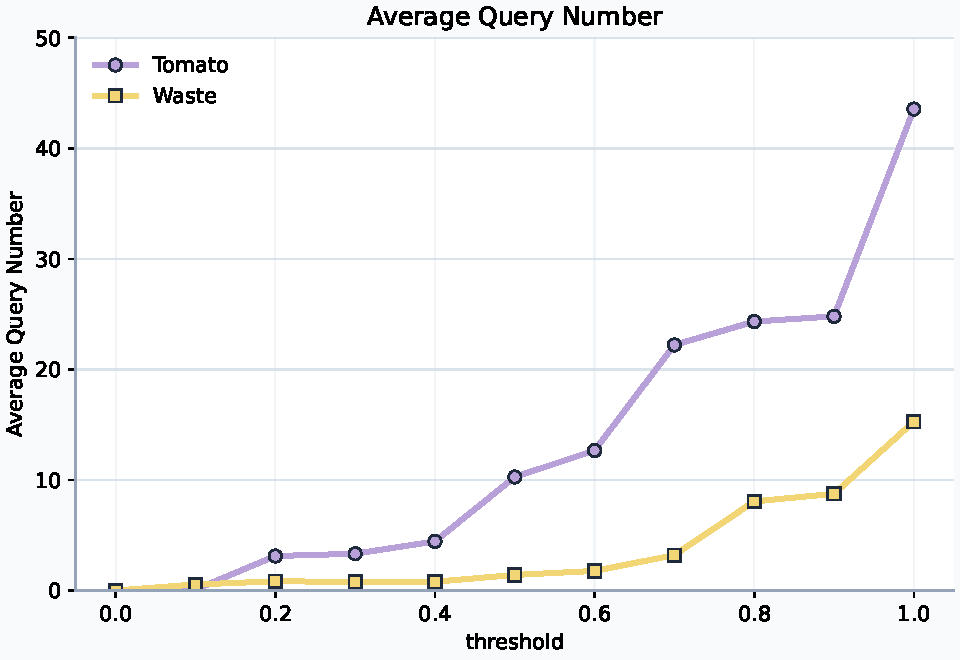
\includegraphics[width=0.3\textwidth]{figures/fig_average_question.pdf}
    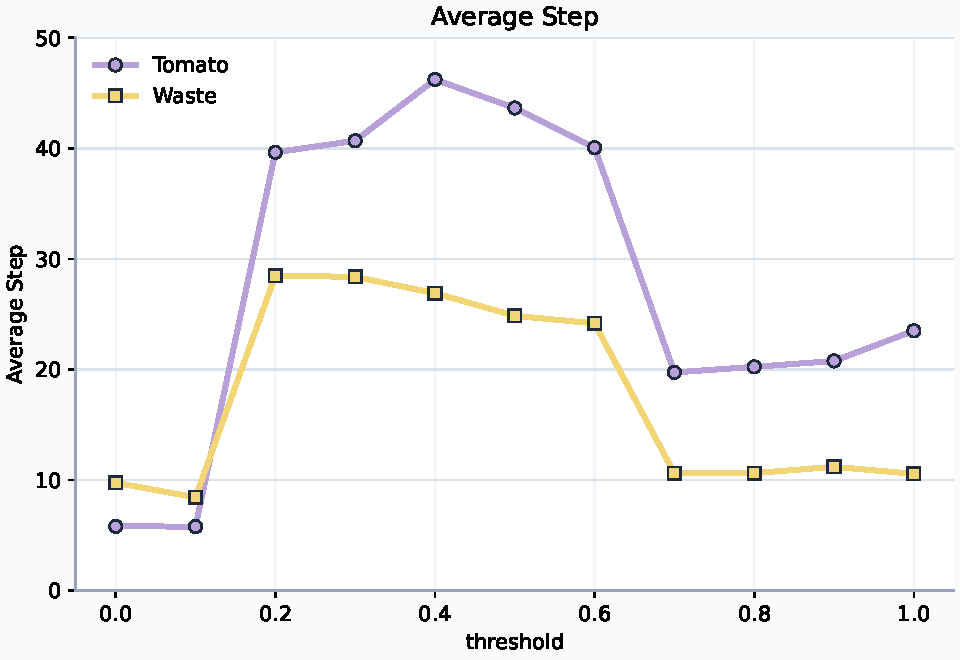
\includegraphics[width=0.3\textwidth]{figures/fig_average_step.pdf}
    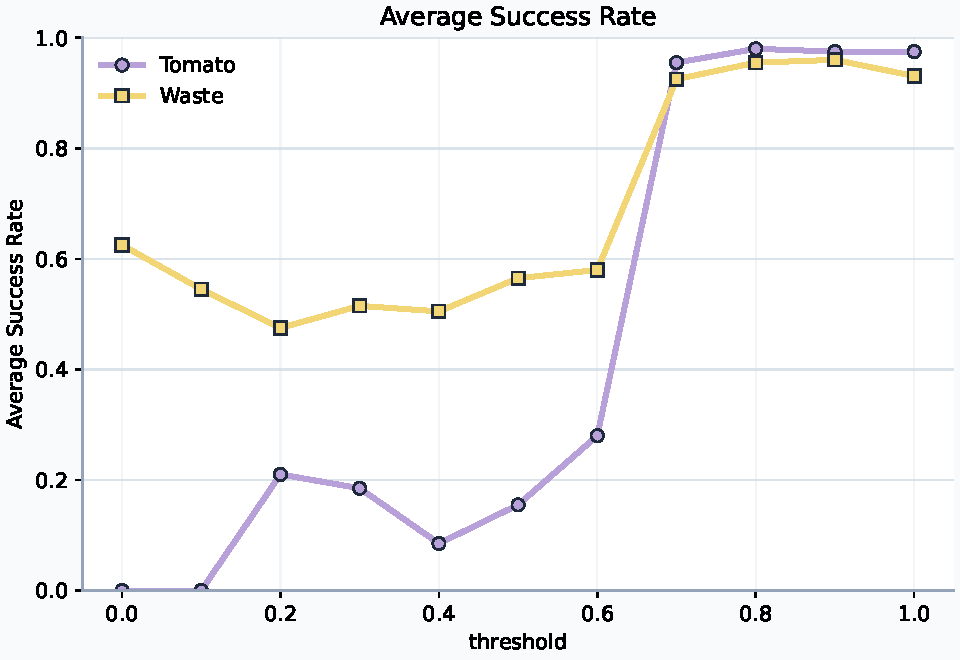
\includegraphics[width=0.3\textwidth]{figures/fig_average_success_rate.pdf}
    \caption{System performance under different confidence thresholds $\tau$. The threshold controls when the robot requests human feedback. Lower thresholds reduce the number of queries but may leave task-relevant uncertainty unresolved, whereas overly high thresholds increase interaction cost without proportional performance gains.}
    \label{fig:sys_tau}
\end{figure*}

We first evaluate the effect of the confidence threshold $\tau$ on system performance. Fig.~\ref{fig:sys_tau} and Table~\ref{tab:sys_tau} report the average number of queries, execution steps, and task success rate under different threshold values.


\begin{table*}[t]
\centering
\caption{System evaluation under different confidence thresholds $\tau$. Success rates are reported as percentages.}
\label{tab:sys_tau}
\small
\setlength{\tabcolsep}{3pt}
\begin{tabular*}{\textwidth}{@{\extracolsep{\fill}}lcccccc}
\toprule
\multirow{2}{*}{$\boldsymbol{\tau}$} & \multicolumn{3}{c}{\textbf{Waste Sorting}} & \multicolumn{3}{c}{\textbf{Tomato Harvesting}} \\
\cmidrule(lr){2-4}\cmidrule(lr){5-7}
& \makecell{\textbf{Success}\\\textbf{Rate (\%)}} & \makecell{\textbf{Avg.}\\\textbf{Queries}} & \makecell{\textbf{Avg.}\\\textbf{Steps}} & \makecell{\textbf{Success}\\\textbf{Rate (\%)}} & \makecell{\textbf{Avg.}\\\textbf{Queries}} & \makecell{\textbf{Avg.}\\\textbf{Steps}} \\
\midrule
0.0 & 62.5 & 0.0  & 9.7  & 0.0  & 0.0  & 5.8  \\
0.1 & 54.5 & 0.6  & 8.4  & 0.0  & 0.1  & 5.8  \\
0.2 & 47.5 & 0.8  & 28.5 & 21.0 & 3.1  & 39.6 \\
0.3 & 51.5 & 0.8  & 28.4 & 18.5 & 3.3  & 40.7 \\
0.4 & 50.5 & 0.8  & 26.9 & 8.5  & 4.4  & 46.2 \\
0.5 & 56.5 & 1.4  & 24.9 & 15.5 & 10.3 & 43.6 \\
0.6 & 58.0 & 1.8  & 24.2 & 28.0 & 12.7 & 40.1 \\
0.7 & 92.5 & 3.2  & 10.6 & 95.5 & 22.2 & 19.7 \\
0.8 & 95.5 & 8.1  & 10.6 & 98.0 & 24.3 & 20.2 \\
0.9 & 96.0 & 8.8  & 11.2 & 97.5 & 24.8 & 20.8 \\
1.0 & 93.1 & 15.3 & 10.6 & 97.5 & 43.5 & 23.5 \\
\bottomrule
\end{tabular*}
\end{table*}


As $\tau$ increases, the average number of queries generally increases in both domains. In waste sorting, increasing $\tau$ from $0.6$ to $0.7$ changes the success rate from $58.0\%$ to $92.5\%$, the average number of queries from $1.8$ to $3.2$, and the average number of execution steps from $24.2$ to $10.6$. In tomato harvesting, the same change results in a success rate increase from $28.0\%$ to $95.5\%$, a query count increase from $12.7$ to $22.2$, and a reduction in execution steps from $40.1$ to $19.7$. For $\tau \geq 0.7$, the success rate remains above $92\%$ in both domains. At $\tau=0.8$, the system achieves success rates of $95.5\%$ and $98.0\%$ in waste sorting and tomato harvesting, respectively. The corresponding average numbers of queries are $8.1$ and $24.3$, and the average numbers of execution steps are $10.6$ and $20.2$. Based on these results, we use $\tau=0.8$ in the remaining experiments.


\begin{figure*}[t!]
    \centering
    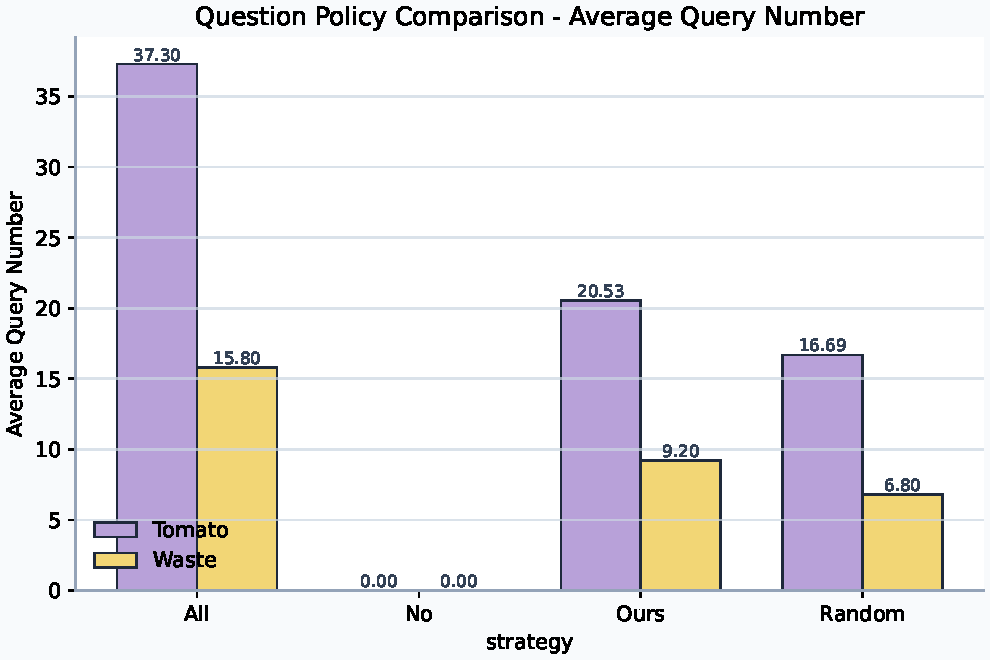
\includegraphics[width=0.3\textwidth]{figures/fig_when_strategy_average_question_domain_compare.pdf}
    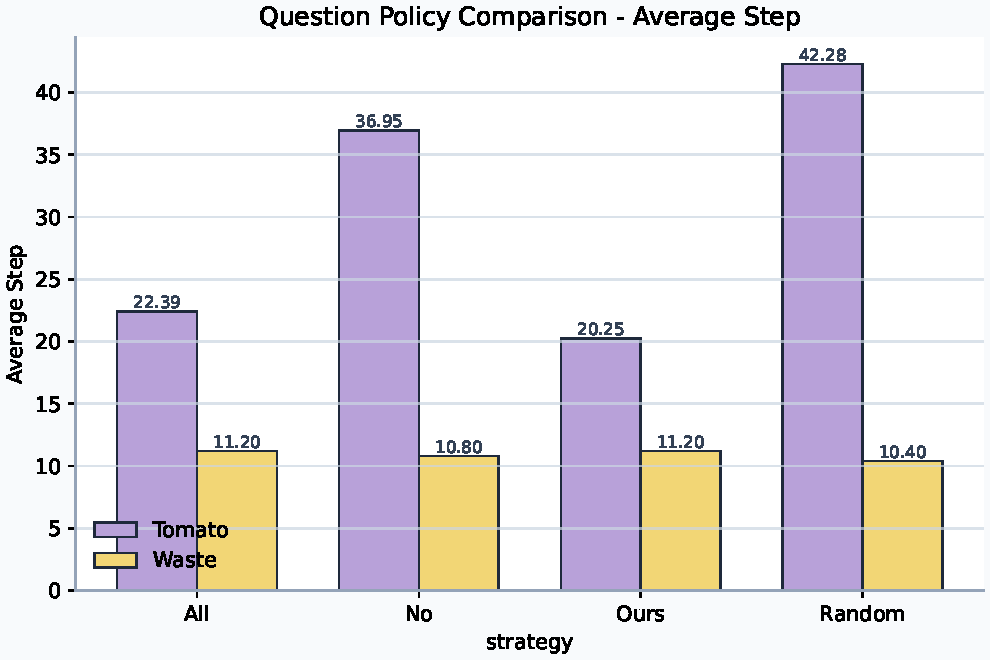
\includegraphics[width=0.3\textwidth]{figures/fig_when_strategy_average_step.pdf}
    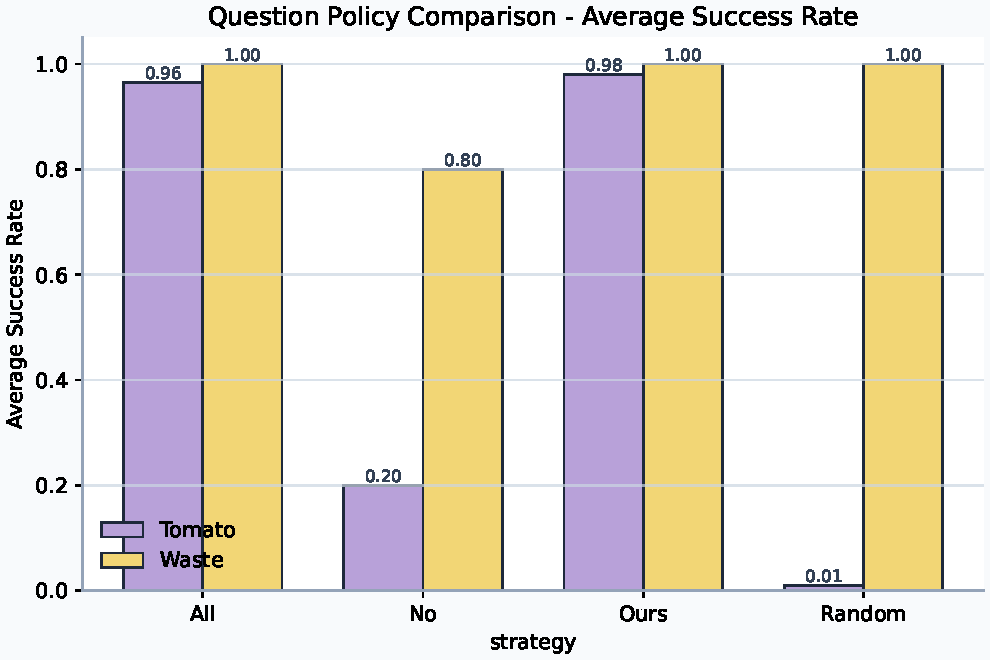
\includegraphics[width=0.3\textwidth]{figures/fig_when_strategy_average_success_rate.pdf}
    \caption{System performance under different querying strategies. The results compare \textbf{All}, \textbf{No}, \textbf{Random}, and \textbf{Ours} in terms of average query count, average execution steps, and task success rate across the two domains.}
    \label{fig:sys_strategy}
\end{figure*}


We next compare four query policies at $\tau=0.8$. \textbf{All} requests feedback whenever a query can be generated. \textbf{No} performs fully autonomous execution without user feedback. \textbf{Random} requests feedback randomly. \textbf{Ours} requests feedback when the confidence of the current belief falls below the threshold and selects the query with the highest expected information gain.


Fig.~\ref{fig:sys_strategy} and Table~\ref{tab:system_eval} summarize the results. In waste sorting, \textbf{All}, \textbf{Random}, and \textbf{Ours} achieve success rates of $100.0\%$, whereas \textbf{No} achieves $80.0\%$. The average numbers of queries are $15.8$, $6.8$, and $9.2$ for \textbf{All}, \textbf{Random}, and \textbf{Ours}, respectively. In tomato harvesting, \textbf{Ours} achieves a success rate of $98.0\%$, compared to $96.5\%$ for \textbf{All}, $20.0\%$ for \textbf{No}, and $1.0\%$ for \textbf{Random}. The corresponding average numbers of queries are $20.5$, $37.3$, $0.0$, and $16.7$. The average numbers of execution steps are $20.2$, $22.4$, $36.9$, and $42.3$, respectively.


\begin{table*}[t]
\centering
\caption{System evaluation under different querying strategies at $\tau=0.8$. \textbf{All} queries whenever feedback is available, \textbf{No} performs fully autonomous execution, \textbf{Random} queries without using belief confidence, and \textbf{Ours} selectively queries based on belief confidence.}
\label{tab:system_eval}
\small
\setlength{\tabcolsep}{4pt}
\begin{tabular*}{\textwidth}{@{\extracolsep{\fill}}lcccccc}
\toprule
\multirow{2}{*}{\textbf{Method}} & \multicolumn{3}{c}{\textbf{Waste Sorting}} & \multicolumn{3}{c}{\textbf{Tomato Harvesting}} \\
\cmidrule(lr){2-4}\cmidrule(lr){5-7}
& \makecell{\textbf{Success}\\\textbf{Rate (\%)}} & \makecell{\textbf{Avg.}\\\textbf{Queries}} & \makecell{\textbf{Avg.}\\\textbf{Steps}} & \makecell{\textbf{Success}\\\textbf{Rate (\%)}} & \makecell{\textbf{Avg.}\\\textbf{Queries}} & \makecell{\textbf{Avg.}\\\textbf{Steps}} \\
\midrule
\textbf{All}    & 100.0 & 15.8 & 11.2 & 96.5 & 37.3 & 22.4 \\
\textbf{No}     & 80.0  & 0.0  & 10.8 & 20.0 & 0.0  & 36.9 \\
\textbf{Random} & 100.0 & 6.8  & 10.4 & 1.0  & 16.7 & 42.3 \\
\textbf{Ours}   & 100.0 & 9.2  & 11.2 & 98.0 & 20.5 & 20.2 \\
\bottomrule
\end{tabular*}
\end{table*}


\subsubsection{System Discussion}~\label{exp:sys_discussion}

The system results show that feedback is most useful when it changes the belief state at decision points that affect future plans. The sharp performance improvement between $\tau=0.6$ and $\tau=0.7$ indicates a transition from acting with unresolved ambiguity to resolving the task-relevant hypotheses before committing to downstream actions. In waste sorting, this often means verifying an uncertain object category before placement. In tomato harvesting, it means disambiguating tomato condition and object existence before the robot commits to picking, scanning, placing, or discarding. Once these high-impact ambiguities are resolved, additional queries provide diminishing returns, which explains why success saturates for $\tau \geq 0.7$ while query frequency continues to increase.

The $\tau=0.0$ condition highlights how task structure shapes the value of feedback. Waste sorting retains $62.5\%$ success because it is a short pick-and-place task in which the main uncertainty is category assignment before bin placement. Tomato harvesting produces $0.0\%$ success because early state estimates guide a longer chain of navigation, detection, picking, scanning, and place/discard decisions. Selective feedback therefore has greater leverage in tomato harvesting: resolving one high-impact state ambiguity can keep several downstream actions aligned with the task goal.

The policy comparison further separates query quantity from query timing. \textbf{All} achieves high success because it resolves nearly every ambiguity, but many of its queries occur after the belief is already sufficiently concentrated for correct planning. \textbf{Ours} avoids these low-value interactions by querying only when the normalized belief entropy indicates that competing frontier states remain plausible. This is why \textbf{Ours} achieves success comparable to \textbf{All} with fewer queries in both domains.

The contrast between \textbf{No}, \textbf{Random}, and \textbf{Ours} shows that feedback timing is as important as feedback availability. Without feedback, early perceptual errors can be promoted into the KB and propagate through symbolic preconditions and effects. Random feedback sometimes supplies useful information in the shorter waste task, but in tomato harvesting its timing often misses the belief ambiguities that determine the next action chain. \textbf{Ours} ties feedback to low-confidence frontier states, so the information arrives when it can still influence the plan.
